\chapter{METODE PENELITIAN}

\section{Jenis Penelitian}
Penelitian ini mendeteksi objek pada sebuah data citra dermoskopi menggunakan metode YOLO. Berdasarkan hal tersebut, penelitian ini termasuk ke dalam penelitian kuantitatif karena data citra dermoskopi berisi data numerik yang terdiri dari matriks dan nilai intensitas piksel. Sehingga pada penelitian ini terdapat perhitungan dan analisis terkait dengan metode dan data yang digunakan untuk mendeteksi kanker kulit pada citra dermoskopi.

\section{Jenis dan Sumber Data}
Penelitian ini menggunakan dataset citra dermoskopi yang berasal dari \textit{ISIC 2019 Challenge}. Dataset \textit{ISIC 2019 Challenge} memiliki 8 jenis kanker kulit, yaitu \textit{Melanoma}, \textit{Actinic Keratosis}, \textit{Basal Cell Carcinoma}, \textit{Squamous Cell Carcinoma}, \textit{Nevus}, \textit{Dermatofibroma}, \textit{Benign Keratosis Lesion}, dan \textit{Vascular Lesion}. Terdapat ribuan data citra kanker kulit, akan tetapi dengan mempertimbangkan perangkat yang digunakan untuk pembentukan model, penelitian ini menggunakan 200 citra pada tiap kelas sehingga terdapat 1600 data citra yang digunakan pada penelitian ini untuk pembentukan model. Sampel citra masing-masing jenis kanker kulit seperti terlihat pada Gambar \ref{fig:dataset}.

\begin{figure}[H]
    \centering
    \begin{tabular}{cccc}
        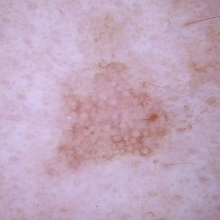
\includegraphics[width=2cm]{../img/Dataset - AK.png}
        &
        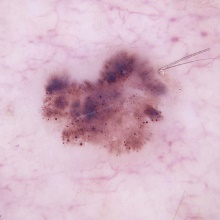
\includegraphics[width=2cm]{../img/Dataset - BCC.png}
        &
        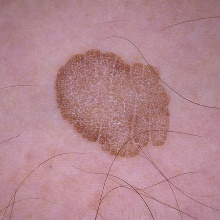
\includegraphics[width=2cm]{../img/Dataset - BKL.png}
        &
        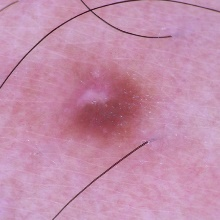
\includegraphics[width=2cm]{../img/Dataset - DF.png}\\
        (a) &(b) &(c) &(d)\\
        \  &\  &\  &\ \\
        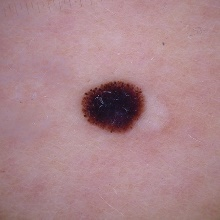
\includegraphics[width=2cm]{../img/Dataset - MEL.png}
        &
        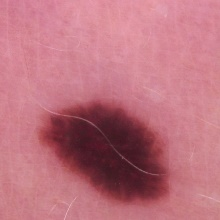
\includegraphics[width=2cm]{../img/Dataset - NV.png}
        &
        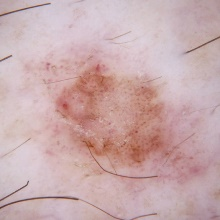
\includegraphics[width=2cm]{../img/Dataset - SCC.png}
        &
        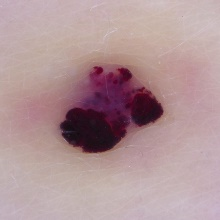
\includegraphics[width=2cm]{../img/Dataset - VASC.png}\\
        (e) &(f) &(g) &(h)\\
    \end{tabular}
    \caption{Dataset citra dermoskopi kanker kulit (a) AK; (b) BCC; (c) BKL; (d) DF; (e) MEL; (f) NV; (g) SCC; (h) VASC;}
    \label{fig:dataset}
\end{figure}

\section{Kerangka Penelitian}
Tahapan dalam melakukan deteksi kanker kulit berdasarkan citra dermoskopi menggunakan YOLO-v7 pada penelitian ini seperti terlihat pada Gambar \ref{fig:flowchart}.

\begin{figure}[H]
    \begin{center}
        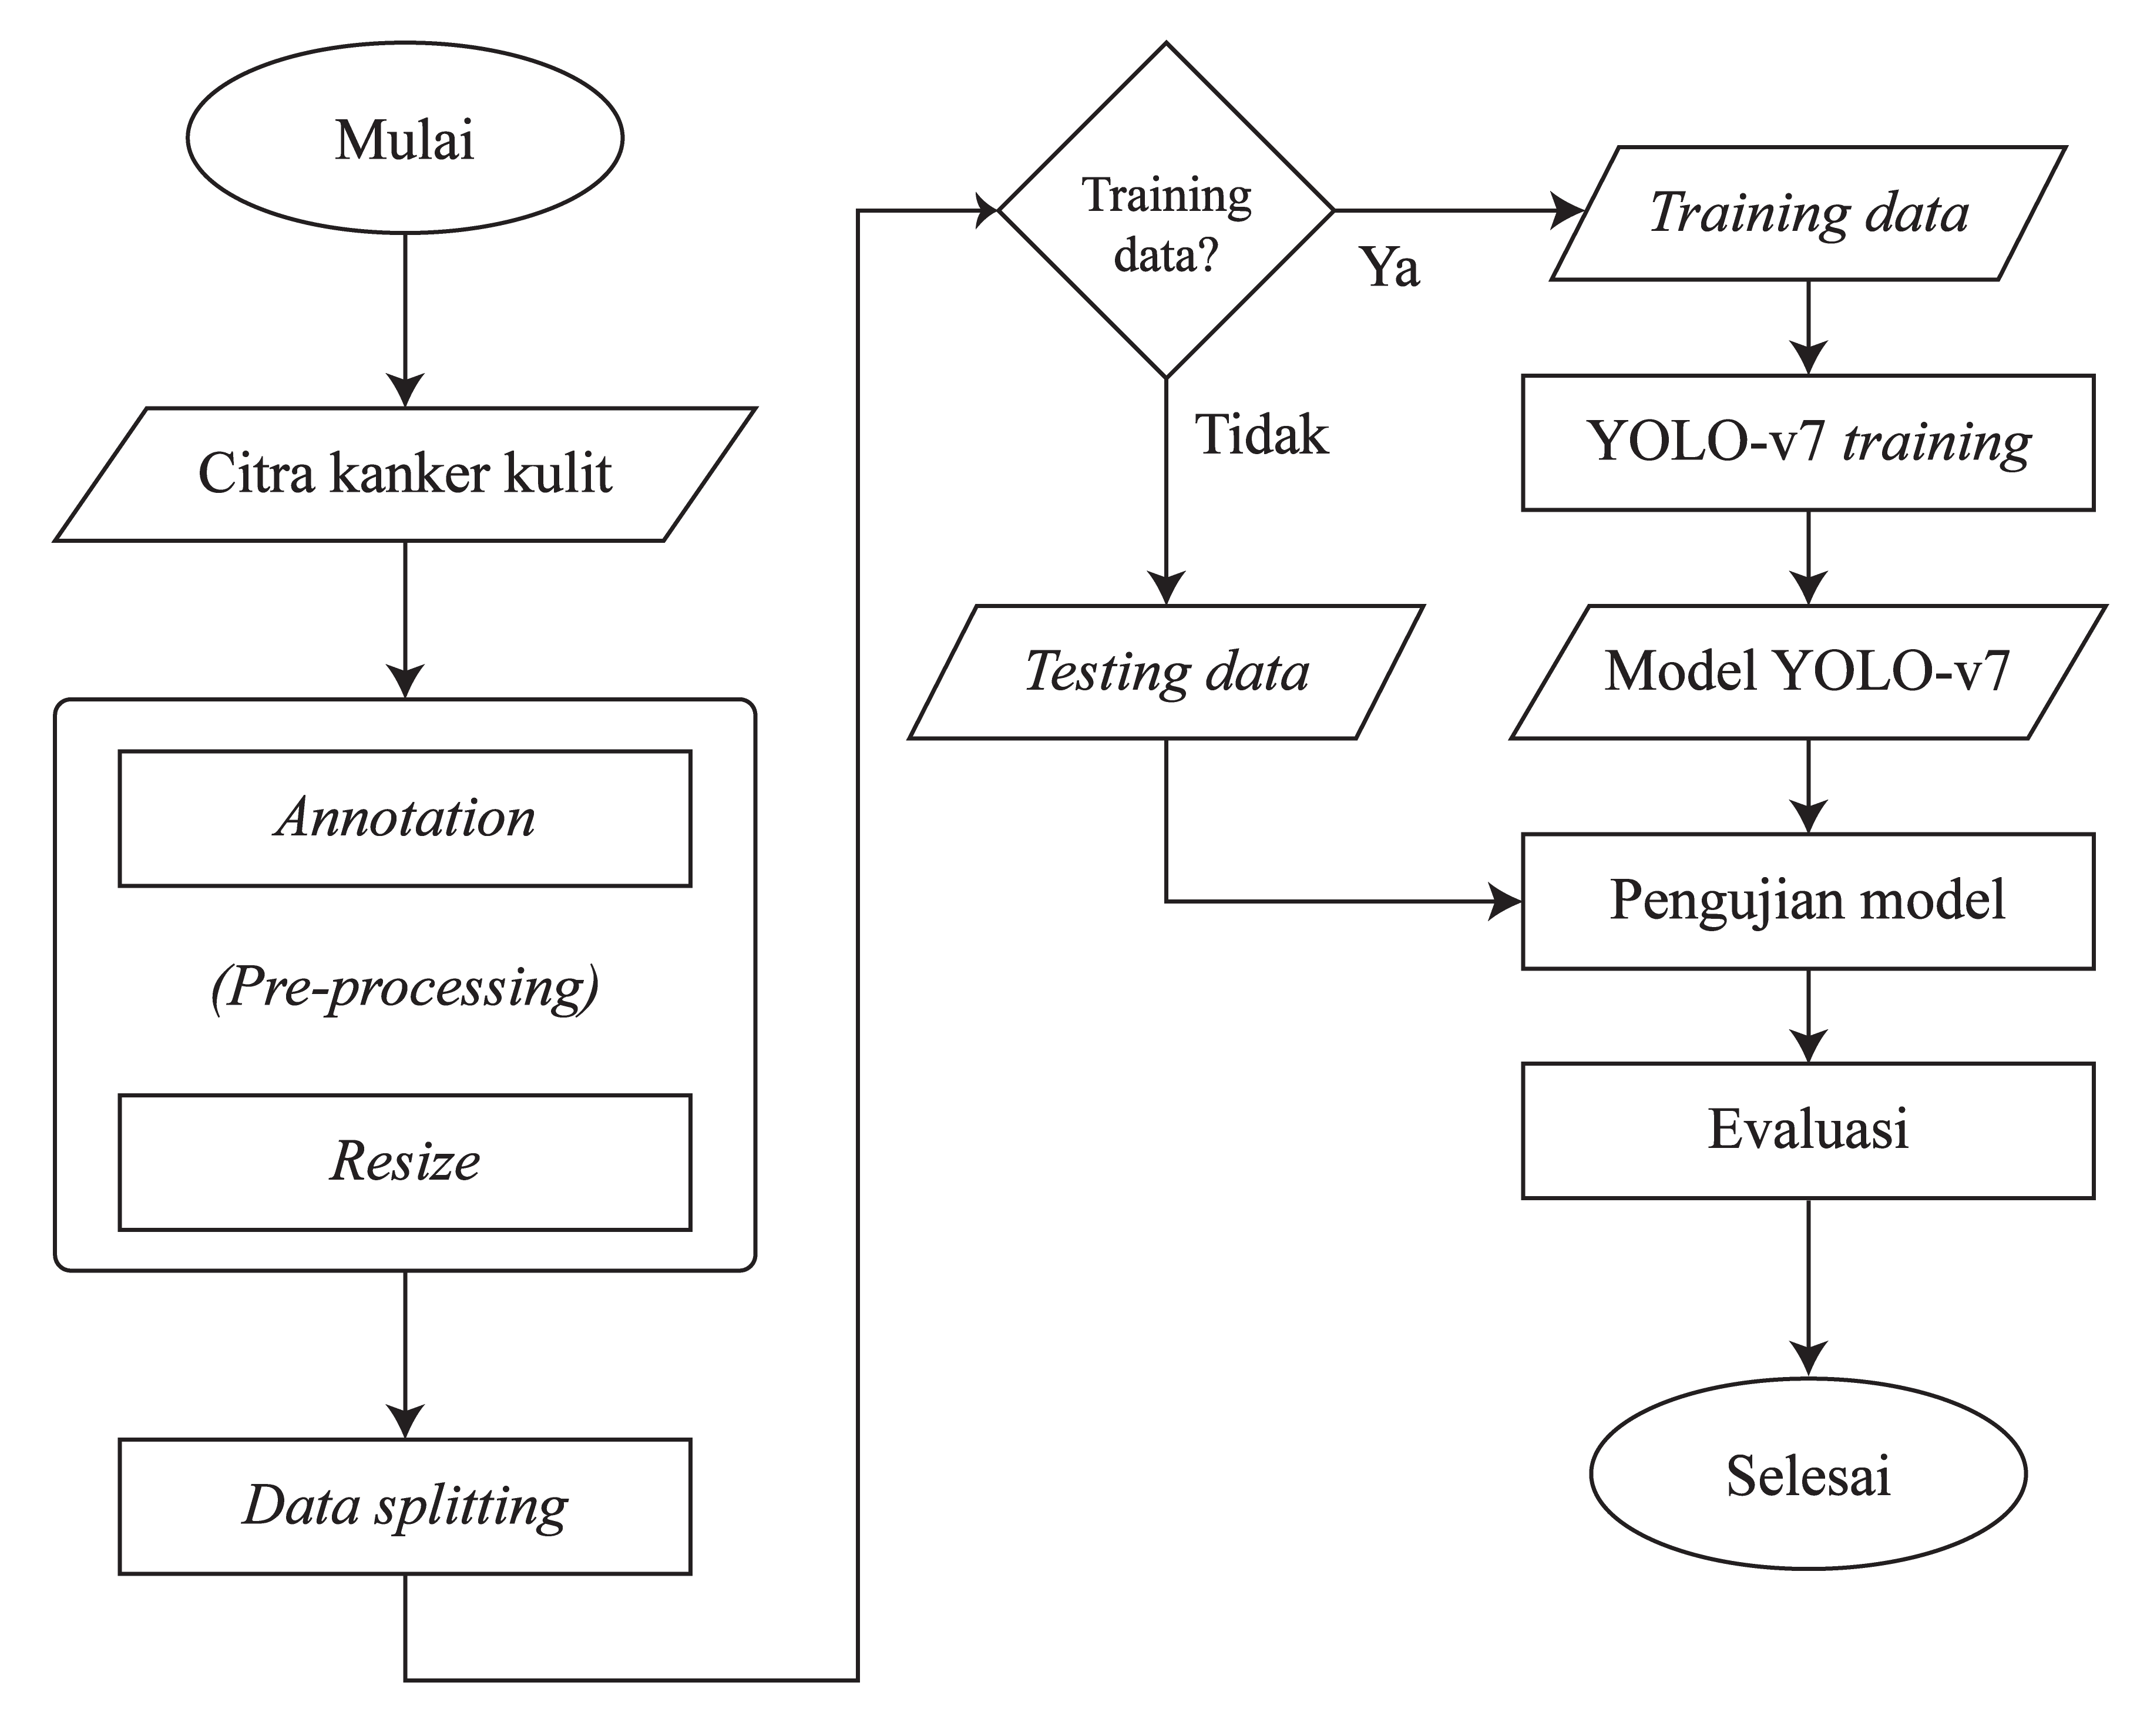
\includegraphics[width=13cm]{../img/Flowchart.png}
        \caption{Diagram alir pada penelitian ini}
        \label{fig:flowchart}
    \end{center}
\end{figure}

Penelitian ini terdiri dari beberapa proses sebagai berikut:
\begin{enumerate}
    \item Tahap \textit{pre-processing} terdiri dari \textit{annotation} dan \textit{resize}. \textit{Annotation} merupakan pemberian kotak pembatas sebuah objek pada sebuah citra. Hal ini dilakukan satu per satu sesuai dengan label yang diberikan dari penyedia dataset, yaitu \textit{ISIC 2019 Challenge}. \textit{Resize} merupakan pengubahan ukuran piksel pada sebuah citra, sehingga penelitian ini melakukan \textit{resize} citra masukan menjadi ukuran $1024\times 1024$, $512\times 512$, dan $256\times 256$. Proses \textit{annotation} dan \textit{resize} seperti terlihat pada Gambar \ref{fig:preprocessing}.
    \begin{figure}[H]
        \centering
        \begin{tabular}{ccc}
            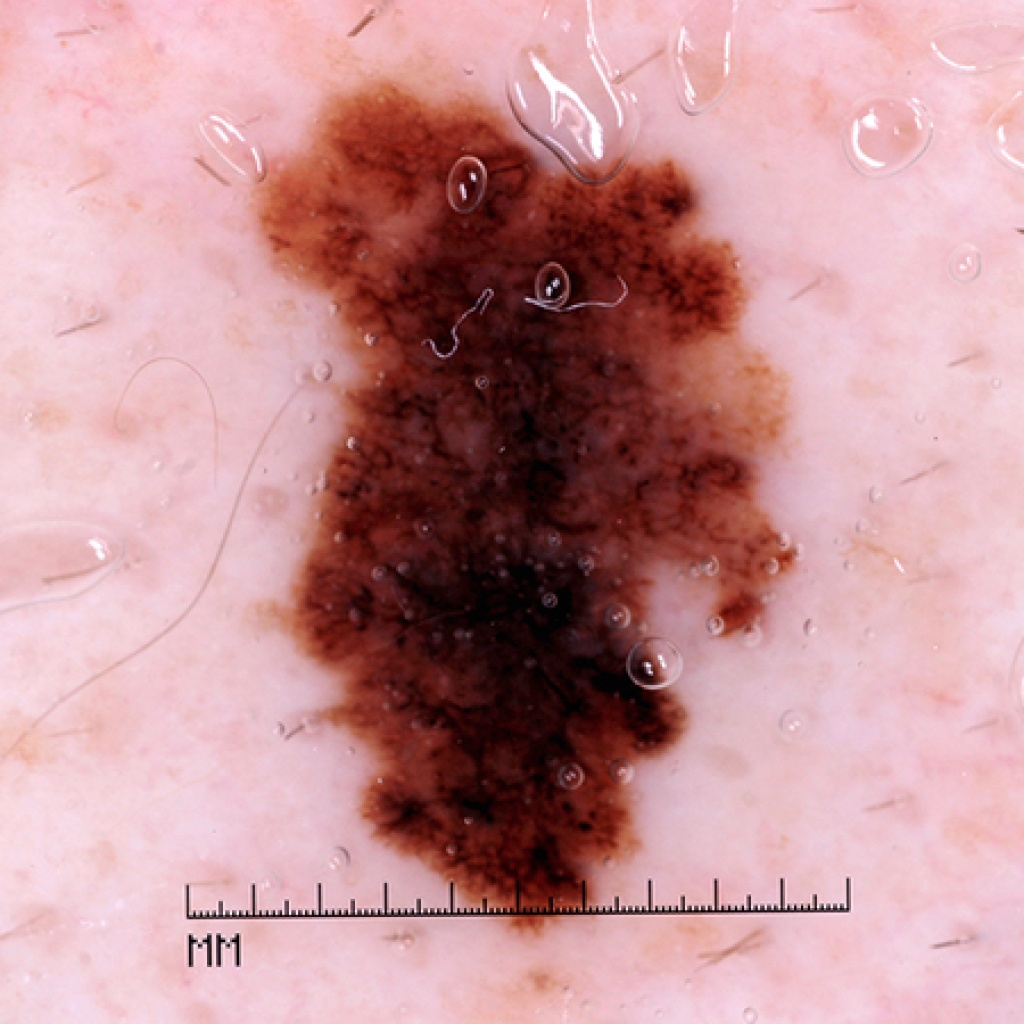
\includegraphics[width=2cm]{../img/Dermoscopy - Latex.jpg}
            &
            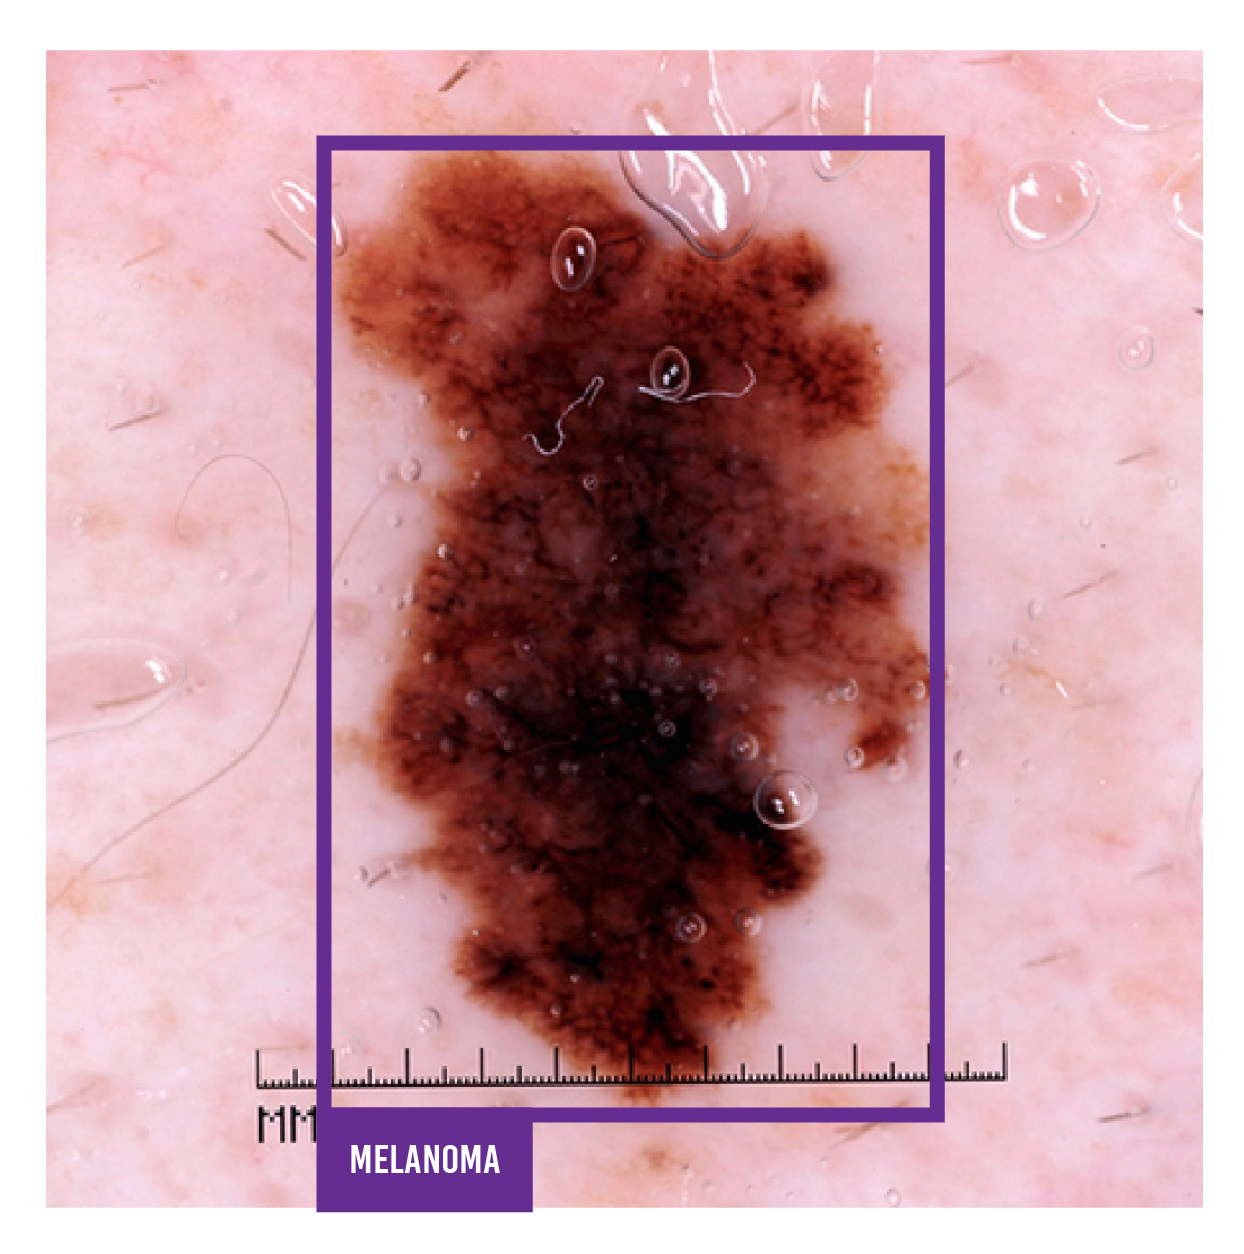
\includegraphics[width=2cm]{../img/Annotation - Latex.png}
            &
            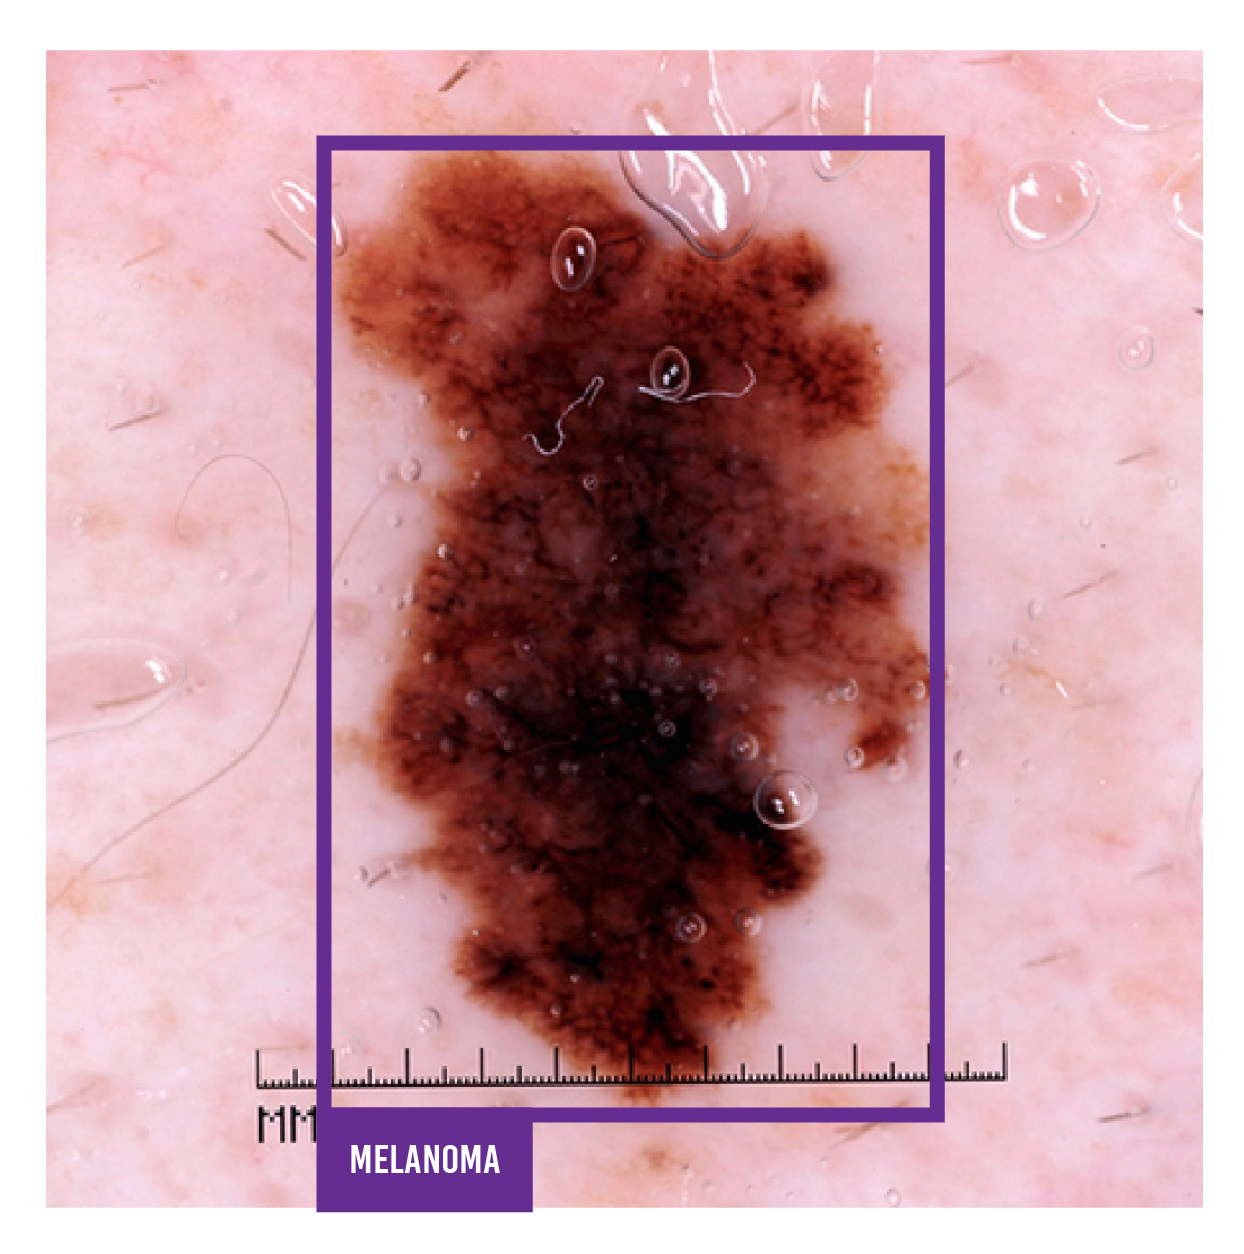
\includegraphics[width=1.5cm]{../img/Annotation - Latex.png}\\
            (a) &(b) &(c)\\
        \end{tabular}
        \caption{Tahap \textit{pre-processing} (a) Citra asli; (b) Citra yang sudah dianotasi; (c) Citra yang sudah diubah ukurannya}
        \label{fig:preprocessing}
    \end{figure}

    \item \textit{Data splitting} merupakan tahap pembagian data. Penelitian ini membagi data menjadi dua, yaitu $90\%$ data untuk proses pelatihan dan $10\%$ data untuk proses pengujian.
    \item Proses pembentukan model YOLO-v7 berdasarkan uji coba \textit{batch size} dan jenis model YOLO-v7. Uji coba \textit{batch size} yang dilakukan adalah sebesar $32$, $64$, dan $128$. Terdapat beberapa jenis YOLO-v7, yaitu YOLO-v7, YOLO-v7-X, YOLO-v7-W6, YOLO-v7-E6, YOLO-v7-D6, dan YOLO-v7-E6E.
    \item Proses pengujian model yaitu tahap model diuji menggunakan \textit{testing data} untuk mendapatkan hasil evaluasi.
    \item Proses evaluasi menggunakan mAP sehingga dilakukan perhitungan mAP berdasarkan \textit{confusion matrix} dan IoU yang didapatkan.
\end{enumerate}

% \begin{figure}[H] 
% \begin{center} 
% \includegraphics[scale=0.58]{Gambar/retina.png}
% \caption{(a) Retina Normal (b) \textit{Mild} DR (c) \textit{Moderate} DR (d) \textit{Severe} DR } 
% Sumber: \citep{aaa}
% \label{gambar13}
% \end{center} 
% \end{figure}

% \vspace{0cm}\noindent
% \begin{table}[H]
% \caption{Tingkat penyakit \textit{diabetic retinopathy}}
% \centering
% \begin{tabular}{|c|c|c|c|}
% \hline
% \textbf{Tingkat} & $\mu\alpha$ & \textbf{h} & \textbf{nv}\\
% \hline
% Normal & 0 & 0 & Tidak \\
% \hline
% \textit{Mild} DR & $>0$ dan $\leq 5$ & 0 & Tidak \\
% \hline
% \textit{Moderate} DR & $>5$ dan $< 15$ & $>0$ dan $<5$ & Tidak \\
% \hline
% \textit{Severe} DR & $\geq 15$ & $\geq 5$ & Ada \\
% \hline
% \end{tabular}
% \label{tabel5}

% Sumber: \citep{aaa}
% \end{table}